% Plantilla creada por Eduardo Mosqueira Rey
%
% Libro online bastante completo para consulta de Latex: http://en.wikibooks.org/wiki/LaTeX/
% Versión en castellano: http://es.wikibooks.org/wiki/Manual_de_LaTeX
\documentclass[12pt, a4paper, titlepage]{article}

\usepackage[spanish]{babel} % Soporte multilenguaje para LaTeX.

\usepackage[a4paper, top=2.5cm, bottom=2.5cm, left=2.5cm, right=2.5cm]{geometry} % Interfaz flexible para definir las dimensiones del documento

\usepackage[utf8]{inputenc} % Aceptar diferentes tipos de codificación de caracteres de entrada (en este caso usamos la codificación Unicode UTF-8)

\usepackage{graphicx} % Soporte aumentado para gráficos 
\usepackage{captdef} %captions personalizadas
\usepackage{rotating}
\begin{document}

%%%%%%%%%%%%%%%%%%%%%%%%%%%%%%%%%%%%%%%%%%%%%%%%%%%%%%%%%%%%%%%%%%%%%%%%%%%%%%%%
% PORTADA
%%%%%%%%%%%%%%%%%%%%%%%%%%%%%%%%%%%%%%%%%%%%%%%%%%%%%%%%%%%%%%%%%%%%%%%%%%%%%%%%

\begin{titlepage}


\includegraphics[width=15cm]{Imagenes/Simbolo_logo_UDC.png}

% Lista de tamaños: \Huge, \huge, \LARGE, \Large, \large, \small, \footnotesize, \tiny
\vspace{3cm}

\begin{center}

\includegraphics[scale=0.3]{Imagenes/1a_Practica_ER_14-15.png}
\end{center}


\begin{flushright}
	
	\LARGE{\textbf{ JoinMe!}}
	
	\LARGE{\textbf{Realización Casos de Uso}}
	
	\large{\textbf{Version 1.0}}
	
\end{flushright}

\vspace{1cm}
\begin{center}
José Antonio López Sebio\\
Pablo Paz Varela\\
Grupo ER-12-03\\
\end{center}

\vspace{2cm}

\begin{center}
	\large{\textbf{Histórico}}
	
    \begin{tabular}{ | p{4cm} | p{2cm} | p{6cm} | p{3cm} |}
    \hline
    \textbf{Fecha} & \textbf{Version} & \textbf{Descripción} & \textbf{Autor} \\ \hline
      15/04/2014 & 1.0 & Primera Revisión & ER-12-03\\ \hline
      &  &  & \\ \hline
     &  & &\\ \hline
    \end{tabular}
\end{center}

\end{titlepage}
\clearpage
%%%%%%%%%%%%%%%%%%%%%%%%%%%%%%%%%%%%%%%%%%%%%%%%%%%%%%%%%%%%%%%%%%%%%%%%%%%%%%%%
% INDICE
%%%%%%%%%%%%%%%%%%%%%%%%%%%%%%%%%%%%%%%%%%%%%%%%%%%%%%%%%%%%%%%%%%%%%%%%
\tableofcontents
\newpage

%%%%%%%%%%%%%%%%%%%%%%%%%%%%%%%%%%%%%%%%%%%%%%%%%%%%%%%%%%%%%%%%%%%%%%%%%%%%%%%%
\section{Introduction}
%%%%%%%%%%%%%%%%%%%%%%%%%%%%%%%%%%%%%%%%%%%%%%%%%%%%%%%%%%%%%%%%%%%%%%%%%%%%%%%%


%**********************************************************
\subsection{Objetivo}
%**********************************************************

Este documento es una visión del sistema empleando diagramas, mostrando así la interacción entre las distintas partes del mismo.

%**********************************************************
\subsection{Ámbito}
%**********************************************************

\textbf{JoinMe!} es una red social, basado en una arquitectura cliente servidor que permite a los usuarios mantener el contacto con sus amigos, y a las empresas anunciarse de una manera más eficiente. 

%**********************************************************
\subsection{Definiciones, Acrónimos y Abreviaturas}
%**********************************************************

Las definiciones, acrónimos y abreviaturas se encuentran el el documento \textit{Glosario}.

%**********************************************************
\subsection{Referencias}
%**********************************************************

\begin{enumerate}
	\item JoinMe! - Glosario
    \item JoinMe! - Modelo de casos de uso
    \item JoinMe! - Especificación suplementaria
    \item JoinMe! - Modelo del dominio
    \item JoinMe! - Arquitectura lógica
    \item JoinMe! - DSS

\end{enumerate}

%%%%%%%%%%%%%%%%%%%%%%%%%%%%%%%%%%%%%%%%%%%%%%%%%%%%%%%%%%%%%%%%%%%%%%%%%%%%%%%%
\section{CU01 - Registrar usuario}
%%%%%%%%%%%%%%%%%%%%%%%%%%%%%%%%%%%%%%%%%%%%%%%%%%%%%%%%%%%%%%%%%%%%%%%%%%%%%%%%

Este caso de uso permite a un futuro usuario poder registrarse en el sistema y así poder acceder a todas las funcionalidades disponibles en \textbf{JoinMe!}. Para ello el usuario tendrá que proporcionar sus datos personales o utilizar un certificado digital como puede ser el DNI-e.

\begin{center}
	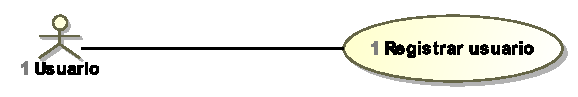
\includegraphics{Imagenes/RegistrarUsuarioCU}
\end{center}

%**********************************************************
\subsection{Flujo de Eventos}
%**********************************************************
El usuario introduce sus datos personales necesarios para el registro o utilizar un certificado digital.

%**********************************************************
\subsection{Diagrama de interacción}
%**********************************************************

En el caso de {\sc registrar usuario } se han identificado las siguientes operaciones:

\begin{itemize}
	\item El usuario introduce sus datos y los envía al sistema mediante la operacion \textbf{registrarUsuario}.
\end{itemize}

\begin{center}
	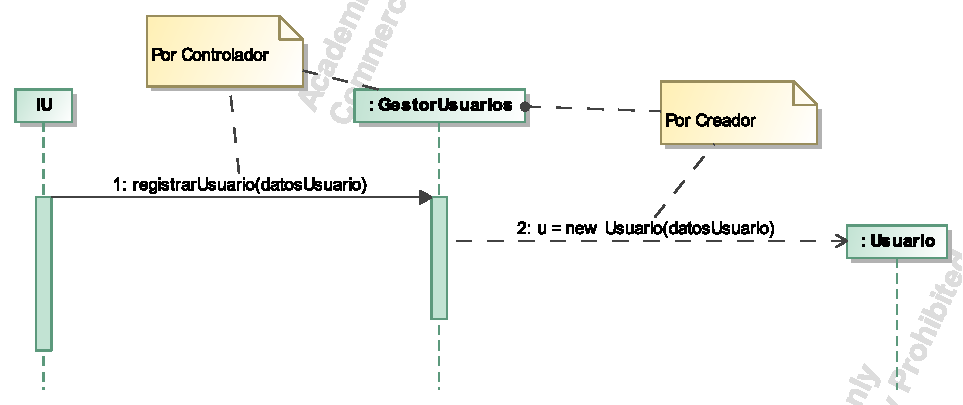
\includegraphics{Imagenes/OperacionRegistrarUsuario.pdf}
\end{center}

%**********************************************************
\subsection{Objetos participantes}
%**********************************************************

\begin{center}

\begin{tabular}{|c|p{14cm}|}
	\hline
	\textbf{Clase} & \textbf{Descripción}\\ \hline
	\textbf{GestorUsuarios} &  Clase que se encarga de realizar las operaciones permitidas sobre los usuarios, tales como registro, modificación y baja.\\ \hline
	\textbf{Usuario} & Clase que representa al usuario. \\ \hline
\end{tabular}

\end{center}

%**********************************************************
\subsection{Diagrama de clases}
%**********************************************************

Se ha optado por realizar un diagrama de clases completo, éste, puede verse en la sección \ref{sec:Diagrama} Diagrama de Clases.
%**********************************************************
\subsection{Requisitos derivados}
%**********************************************************

\begin{itemize}
	\item Recuperación robusta cuando el usuario inserta datos incorrectos.
	\item Información por pantalla en caso de error.
\end{itemize}

%%%%%%%%%%%%%%%%%%%%%%%%%%%%%%%%%%%%%%%%%%%%%%%%%%%%%%%%%%%%%%%%%%%%%%%%%%%%%%%%
\section{CU03 - Aceptar solicitud de amistad}
%%%%%%%%%%%%%%%%%%%%%%%%%%%%%%%%%%%%%%%%%%%%%%%%%%%%%%%%%%%%%%%%%%%%%%%%%%%%%%%%


Este caso de uso representa la acción de aceptar una solicitud de amistad enviada por otro usuario de la red social \textbf{JoinMe!} que quiere añadir al usuario en cuestión a su círculo de amistades.

\begin{center}
	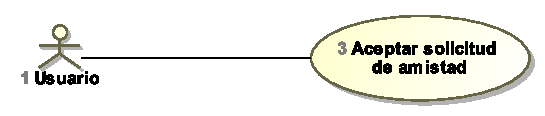
\includegraphics{Imagenes/AceptarSolicitudAmistadCU.pdf}
\end{center}
%**********************************************************
\subsection{Flujo de Eventos}
%**********************************************************

El usuario acepta la solicitud de amistad que tiene en su bandeja de solicitudes haciendo click en el botón oportuno.

%**********************************************************
\subsection{Diagrama de interacción}
%**********************************************************

En el caso de {\sc aceptar solicitud de amistad } se han identificado las siguientes operaciones:

\begin{itemize}
	\item El usuario acepta la petición de amistad a través de la operación \textbf{aceptarAmistad}.
	\item El sistema registra la aceptación y añade el amigo a lista de amigos con la operación \textbf{aceptarAmigo}.
\end{itemize}

\begin{center}
	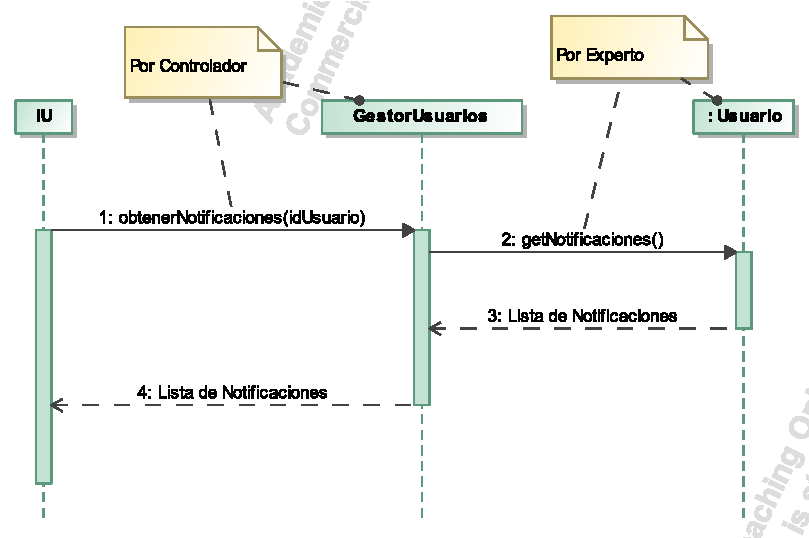
\includegraphics{Imagenes/OperacionObtenerNotificaciones}
\end{center}

\begin{center}
	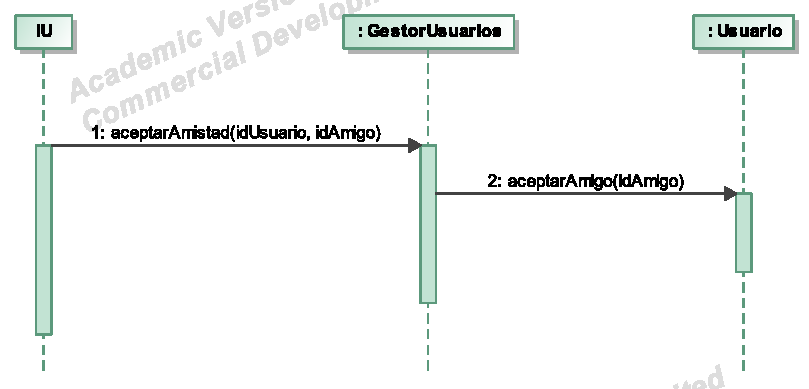
\includegraphics{Imagenes/OperacionAceptarAmistad}
\end{center}

\begin{center}
	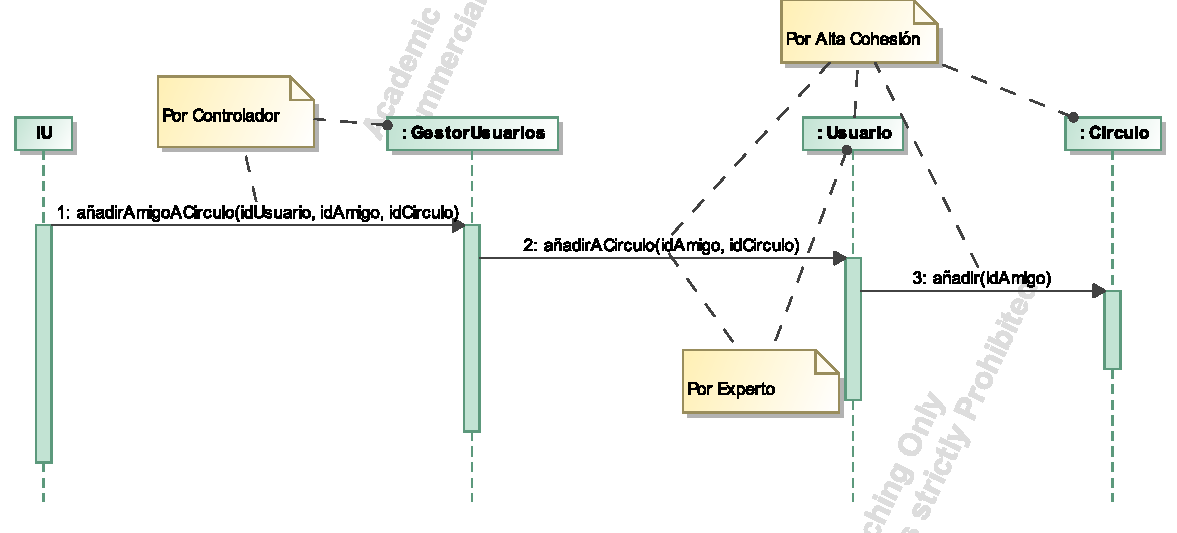
\includegraphics{Imagenes/OperacionAnadirAmigoACirculo}
\end{center}



%**********************************************************
\subsection{Objetos participantes}
%**********************************************************

\begin{center}

\begin{tabular}{|c|p{14cm}|}
	\hline
	\textbf{Clase} & \textbf{Descripción}\\ \hline
	\textbf{GestorUsuarios} &  Clase que se encarga de realizar las operaciones permitidas sobre los usuarios, tales como registro, modificación y baja.\\ \hline
	\textbf{Usuario} & Clase que representa al usuario. \\ \hline
\end{tabular}

\end{center}


%**********************************************************
\subsection{Diagrama de clases}
%**********************************************************
Se ha optado por realizar un diagrama de clases completo, éste, puede verse en la sección \ref{sec:Diagrama} Diagrama de Clases.
%**********************************************************
\subsection{Requisitos derivados}
%**********************************************************
\begin{itemize}
	\item Recuperación robusta en caso de fallo del sistema.
	\item Información por pantalla en caso de error.
\end{itemize}

%%%%%%%%%%%%%%%%%%%%%%%%%%%%%%%%%%%%%%%%%%%%%%%%%%%%%%%%%%%%%%%%%%%%%%%%%%%%%%%%
\section{CU04 - Rechazar solicitud de amistad}
%%%%%%%%%%%%%%%%%%%%%%%%%%%%%%%%%%%%%%%%%%%%%%%%%%%%%%%%%%%%%%%%%%%%%%%%%%%%%%%%

Caso de uso que representa la acción de rechazar una petición de amistad enviada anteriormente por otro usuario de \textbf{JoinMe!}.

\begin{center}
	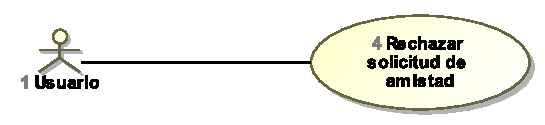
\includegraphics{Imagenes/RechazarSolicitudAmistadCU}
\end{center}
%**********************************************************
\subsection{Flujo de Eventos}
%**********************************************************

El usuario rechaza la solicitud de amistad que tiene en la bandeja de solicitudes de amistad haciendo uso del botón de rechazar solicitud.

%**********************************************************
\subsection{Diagrama de interacción}
%**********************************************************
En el caso de {\sc rechazar solicitud de amistad } se han identificado las siguientes operaciones:

\begin{itemize}
	\item El usuario rechazar la solicitud con la operación \textbf{rechazarAmistad}.
\end{itemize}

\begin{center}
	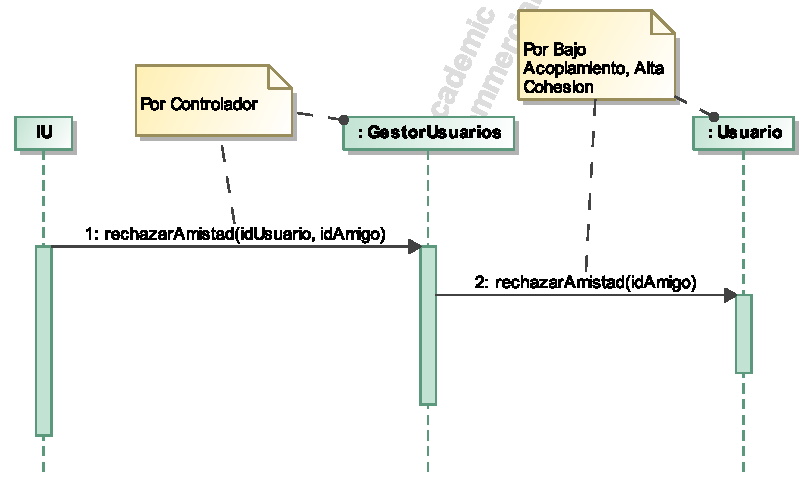
\includegraphics{Imagenes/OperacionRechazarAmistad}
\end{center}

%**********************************************************
\subsection{Objetos participantes}
%**********************************************************
\begin{center}

\begin{tabular}{|c|p{14cm}|}
	\hline
	\textbf{Clase} & \textbf{Descripción}\\ \hline
	\textbf{GestorUsuarios} &  Clase que se encarga de realizar las operaciones permitidas sobre los usuarios, tales como registro, modificación y baja.\\ \hline
	\textbf{Usuario} & Clase que representa al usuario. \\ \hline
\end{tabular}

\end{center}


%**********************************************************
\subsection{Diagrama de clases}
%**********************************************************
Se ha optado por realizar un diagrama de clases completo, éste, puede verse en la sección \ref{sec:Diagrama} Diagrama de Clases.
%**********************************************************
\subsection{Requisitos derivados}
%**********************************************************

\begin{itemize}
	\item Recuperación robusta cuando el usuario inserta datos incorrectos.
	\item Información por pantalla en caso de error.
\end{itemize}

%%%%%%%%%%%%%%%%%%%%%%%%%%%%%%%%%%%%%%%%%%%%%%%%%%%%%%%%%%%%%%%%%%%%%%%%%%%%%%%%
\section{CU05 - Ver amigos}
%%%%%%%%%%%%%%%%%%%%%%%%%%%%%%%%%%%%%%%%%%%%%%%%%%%%%%%%%%%%%%%%%%%%%%%%%%%%%%%%


Caso de uso que representa la opción de listar todos los amigos que tiene un usuario en la red social.

\begin{center}
	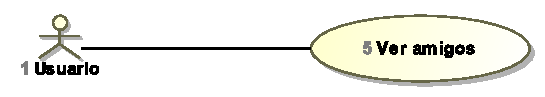
\includegraphics{Imagenes/VerAmigosCU.pdf}
\end{center}
%**********************************************************
\subsection{Flujo de Eventos}
%**********************************************************

El usuario mediante la opción disponible en la interfaz, solicita consultar su lista de amigos.

%**********************************************************
\subsection{Diagrama de interacción}
%**********************************************************

En el caso de {\sc ver amigos } se han identificado las siguientes operaciones:

\begin{itemize}
	\item El usuario obtiene la lista de amigos haciendo uso de la operación \textbf{obtenerListaAmigos}.
\end{itemize}

\begin{center}
	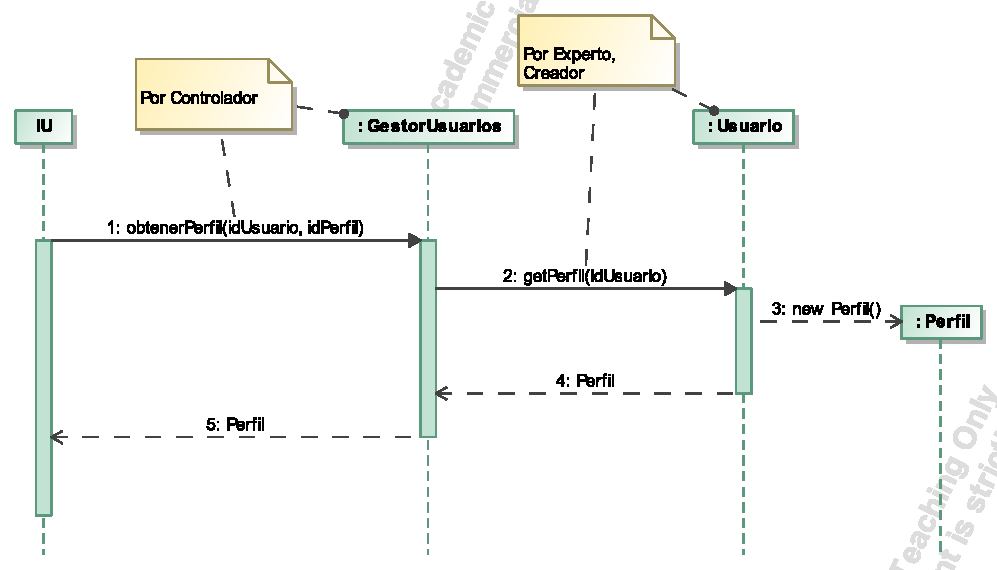
\includegraphics{Imagenes/OperacionObtenerPerfil}
\end{center}

\begin{center}
	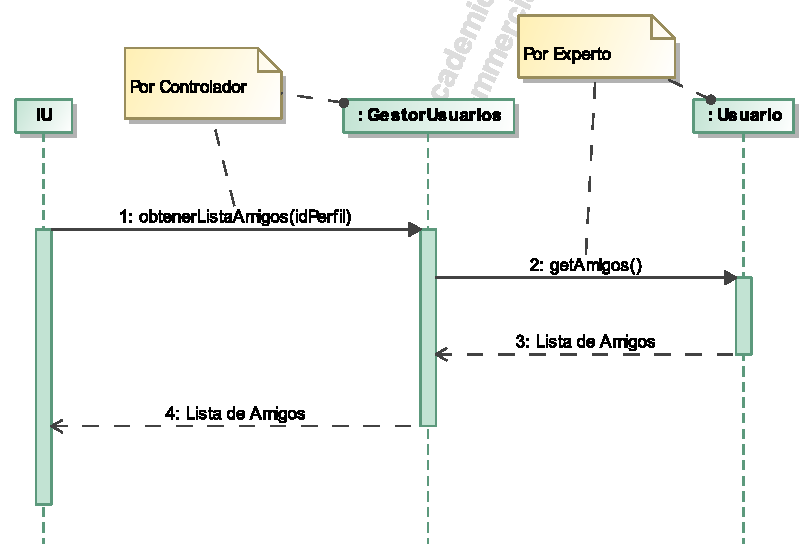
\includegraphics{Imagenes/OperacionObtenerListaAmigos}
\end{center}

\begin{center}
	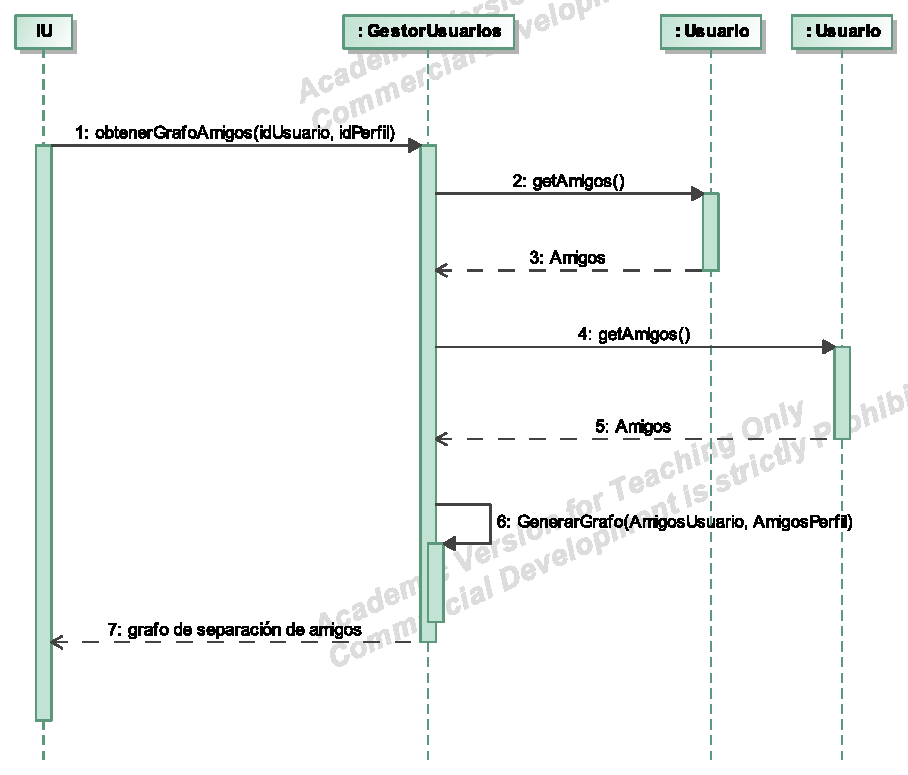
\includegraphics{Imagenes/OperacionObtenerGrafoAmigos}
\end{center}

%**********************************************************
\subsection{Objetos participantes}
%**********************************************************

\begin{center}
\begin{tabular}{|c|p{14cm}|}
	\hline
	\textbf{Clase} & \textbf{Descripción}\\ \hline
	\textbf{GestorUsuarios} &  Clase que se encarga de realizar las operaciones permitidas sobre los usuarios, tales como registro, modificación y baja.\\ \hline
	\textbf{Usuario} & Clase que representa al usuario. \\ \hline
\end{tabular}

\end{center}


%**********************************************************
\subsection{Diagrama de clases}
%**********************************************************
Se ha optado por realizar un diagrama de clases completo, éste, puede verse en la sección \ref{sec:Diagrama} Diagrama de Clases.
%**********************************************************
\subsection{Requisitos derivados}
%**********************************************************

\begin{itemize}
	\item Recuperación robusta cuando el usuario inserta datos incorrectos.
	\item Información por pantalla en caso de error.
\end{itemize}

%%%%%%%%%%%%%%%%%%%%%%%%%%%%%%%%%%%%%%%%%%%%%%%%%%%%%%%%%%%%%%%%%%%%%%%%%%%%%%%%
\section{CU06 - Enviar solicitud de amistad}
%%%%%%%%%%%%%%%%%%%%%%%%%%%%%%%%%%%%%%%%%%%%%%%%%%%%%%%%%%%%%%%%%%%%%%%%%%%%%%%%

Caso de uso que representa la funcionalidad de enviar una solicitud a otro usuario de la res social que deseamos tener entre nuestros contactos en la red.

\begin{center}
	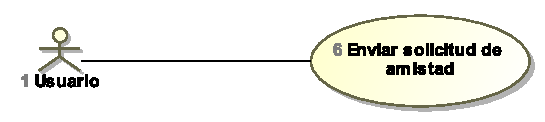
\includegraphics{Imagenes/EnviarSolicitudAmistadCU.pdf}
\end{center}

%**********************************************************
\subsection{Flujo de Eventos}
%**********************************************************

El usuario, envía una solicitud de amistad haciendo click en el botón de enviar solicitud que está en la interfaz del perfil del usuario que desea agregar.

%**********************************************************
\subsection{Diagrama de interacción}
%**********************************************************
En el caso de {\sc enviar solicitud de amistad } se han identificado las siguientes operaciones:

\begin{itemize}
	\item El usuario envía la solicitud de amistad al otro usuario haciendo uso de la operación \textbf{solicitarAmistad}.
\end{itemize}

\begin{center}
	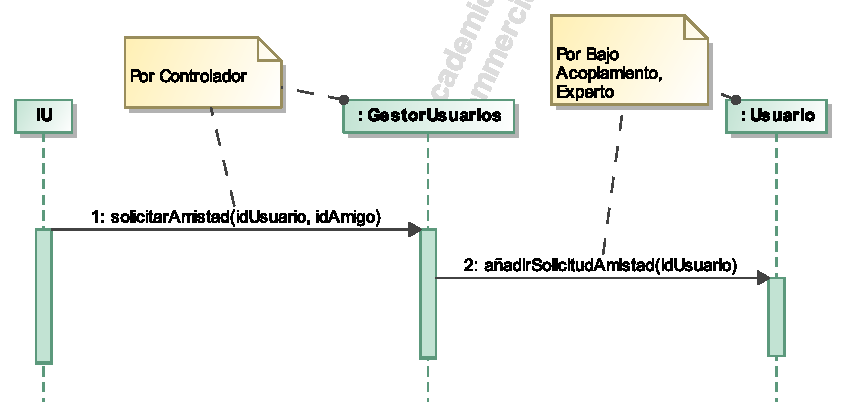
\includegraphics{Imagenes/OperacionSolicitarAmistad}
\end{center}
%**********************************************************
\subsection{Objetos participantes}
%**********************************************************

\begin{center}

\begin{tabular}{|c|p{14cm}|}
	\hline
	\textbf{Clase} & \textbf{Descripción}\\ \hline
	\textbf{GestorUsuarios} &  Clase que se encarga de realizar las operaciones permitidas sobre los usuarios, tales como registro, modificación y baja.\\ \hline
	\textbf{Usuario} & Clase que representa al usuario. \\ \hline
\end{tabular}

\end{center}

%**********************************************************
\subsection{Diagrama de clases}
%**********************************************************
Se ha optado por realizar un diagrama de clases completo, éste, puede verse en la sección \ref{sec:Diagrama} Diagrama de Clases.
%**********************************************************
\subsection{Requisitos derivados}
%**********************************************************

\begin{itemize}
	\item Recuperación robusta cuando el usuario inserta datos incorrectos.
	\item Información por pantalla en caso de error.
\end{itemize}

%%%%%%%%%%%%%%%%%%%%%%%%%%%%%%%%%%%%%%%%%%%%%%%%%%%%%%%%%%%%%%%%%%%%%%%%%%%%%%%%
\section{CU011 - Crear entrada}
%%%%%%%%%%%%%%%%%%%%%%%%%%%%%%%%%%%%%%%%%%%%%%%%%%%%%%%%%%%%%%%%%%%%%%%%%%%%%%%%


Este caso de uso muestra la funcionalidad de crear una entrada que será publicada en la red social. Una entrada que podrá contener, imágenes o vídeos y podrá ser comentada por otros usuarios.

\begin{center}
	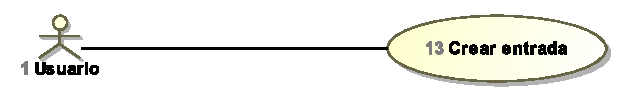
\includegraphics{Imagenes/CrearEntradaCU.pdf}
\end{center}

%**********************************************************
\subsection{Flujo de Eventos}
%**********************************************************


%**********************************************************
\subsection{Diagrama de interacción}
%**********************************************************

En el caso de {\sc crear entrada} se han identificado las siguientes operaciones:

\begin{itemize}
	\item 
\end{itemize}

\begin{center}
	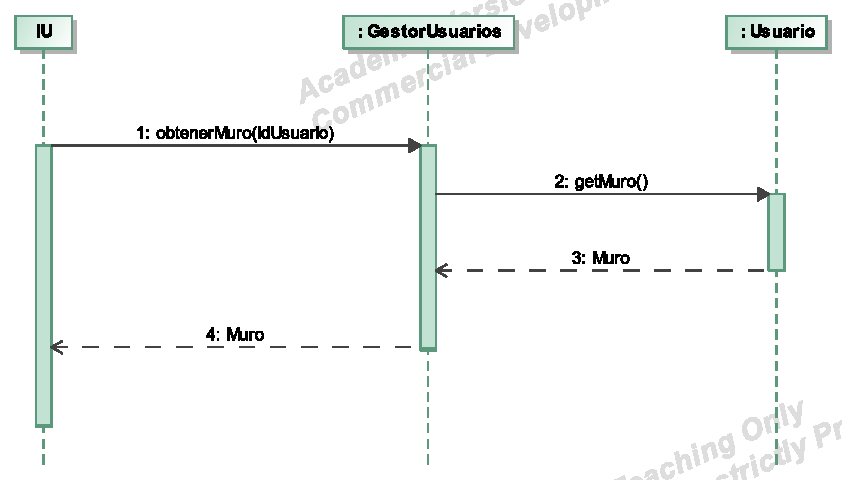
\includegraphics{Imagenes/OperacionObtenerMuro}
\end{center}

\begin{center}
	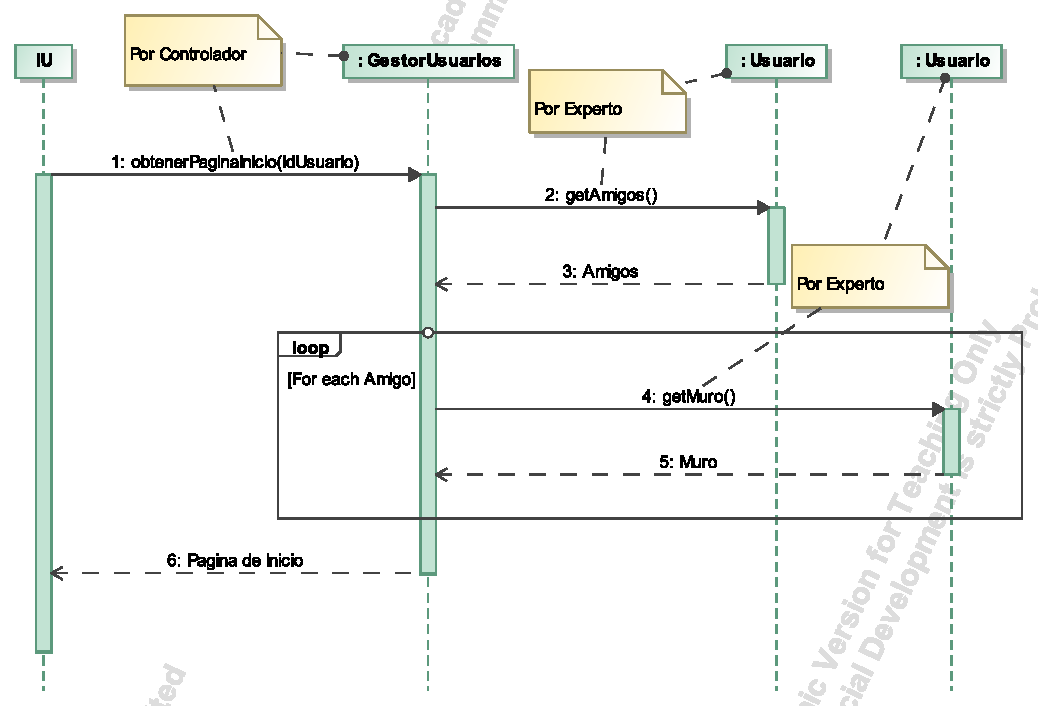
\includegraphics{Imagenes/OperacionObtenerPaginaInicio}
\end{center}

\begin{center}
	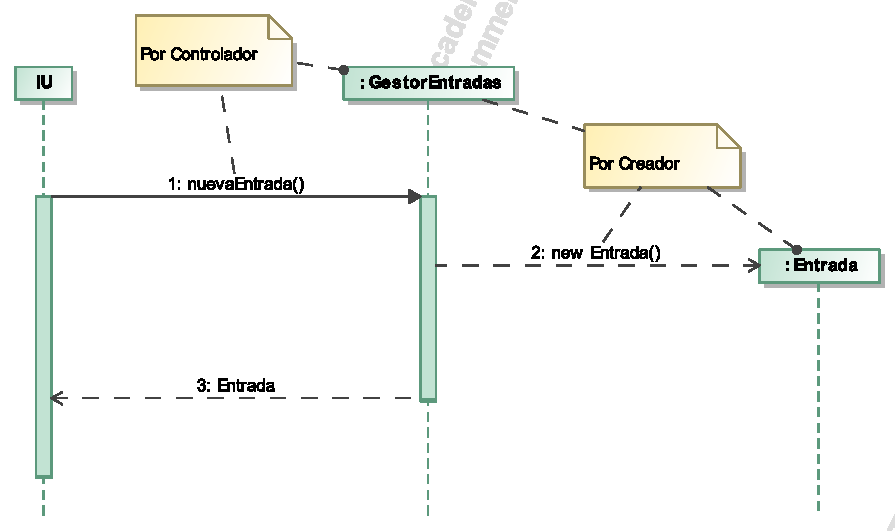
\includegraphics{Imagenes/OperacionNuevaEntrada.pdf}
\end{center}

\begin{center}
	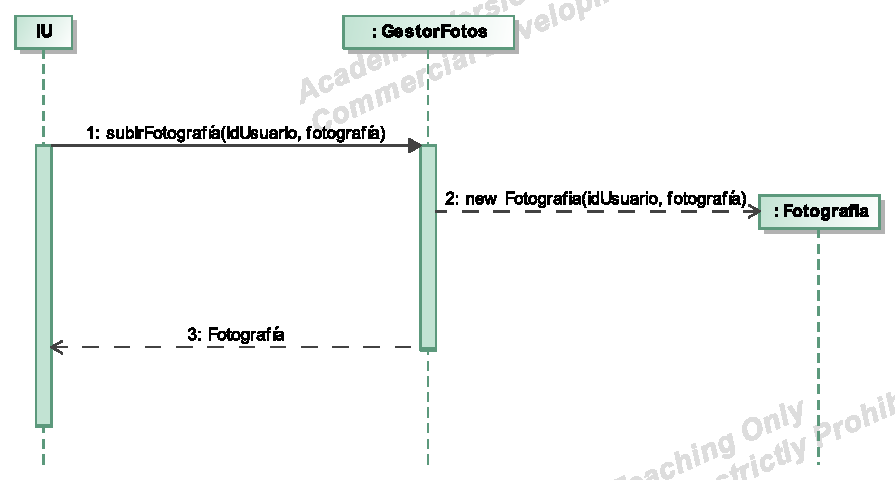
\includegraphics{Imagenes/OperacionSubirFotografia}
\end{center}

\begin{center}
	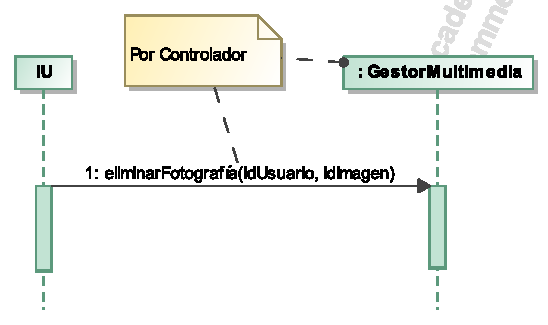
\includegraphics{Imagenes/OperacionEliminarFotografia}
\end{center}

\begin{center}
	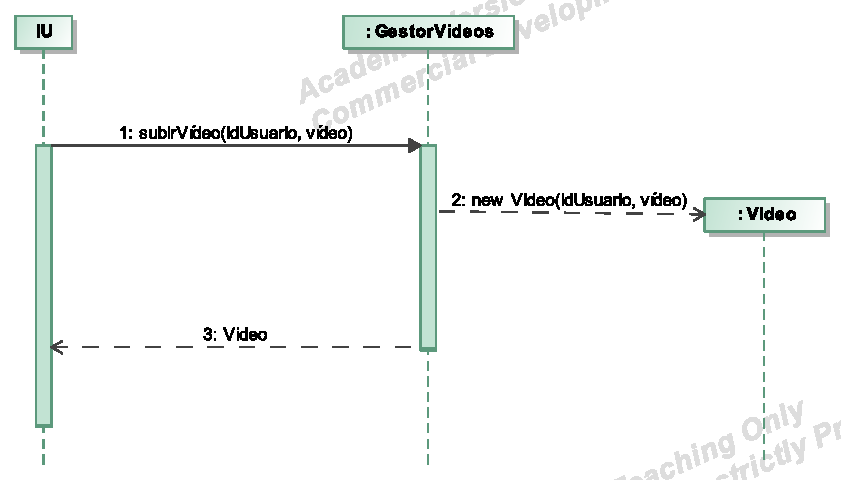
\includegraphics{Imagenes/OperacionSubirVideo}
\end{center}

\begin{center}
	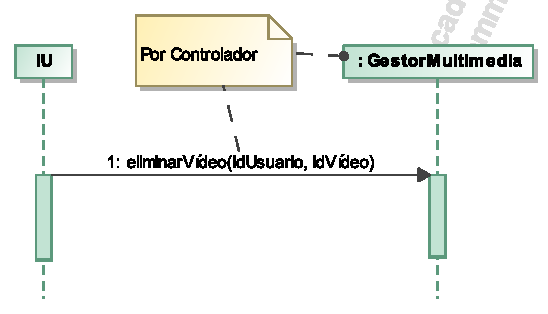
\includegraphics{Imagenes/OperacionEliminarVideo}
\end{center}

\begin{center}
	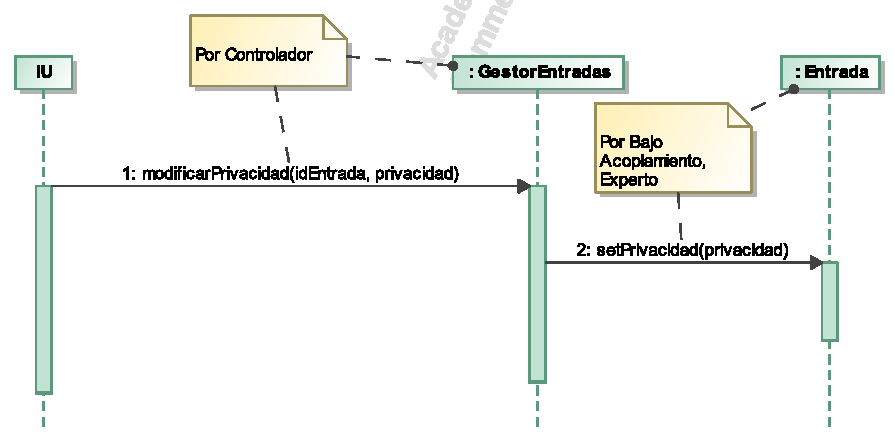
\includegraphics{Imagenes/OperacionModificarPrivacidad}
\end{center}

\begin{center}
	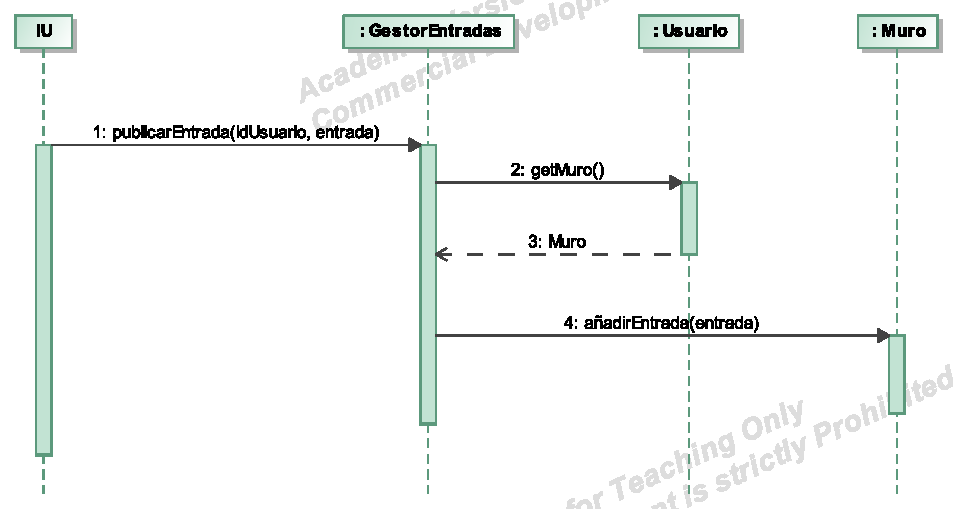
\includegraphics{Imagenes/OperacionPublicarEntrada.pdf}
\end{center}
%**********************************************************
\subsection{Objetos participantes}
%**********************************************************

\begin{center}

\begin{tabular}{|c|p{14cm}|}
	\hline
	\textbf{Clase} & \textbf{Descripción}\\ \hline
\end{tabular}

\end{center}

%**********************************************************
\subsection{Diagrama de clases}
%**********************************************************
Se ha optado por realizar un diagrama de clases completo, éste, puede verse en la sección \ref{sec:Diagrama} Diagrama de Clases.
%**********************************************************
\subsection{Requisitos derivados}
%**********************************************************

\begin{itemize}
	\item Recuperación robusta cuando el usuario inserta datos incorrectos.
	\item Información por pantalla en caso de error.
\end{itemize}

\newpage
\section{Diagrama de clases}\label{sec:Diagrama}

	

\begin{center}
	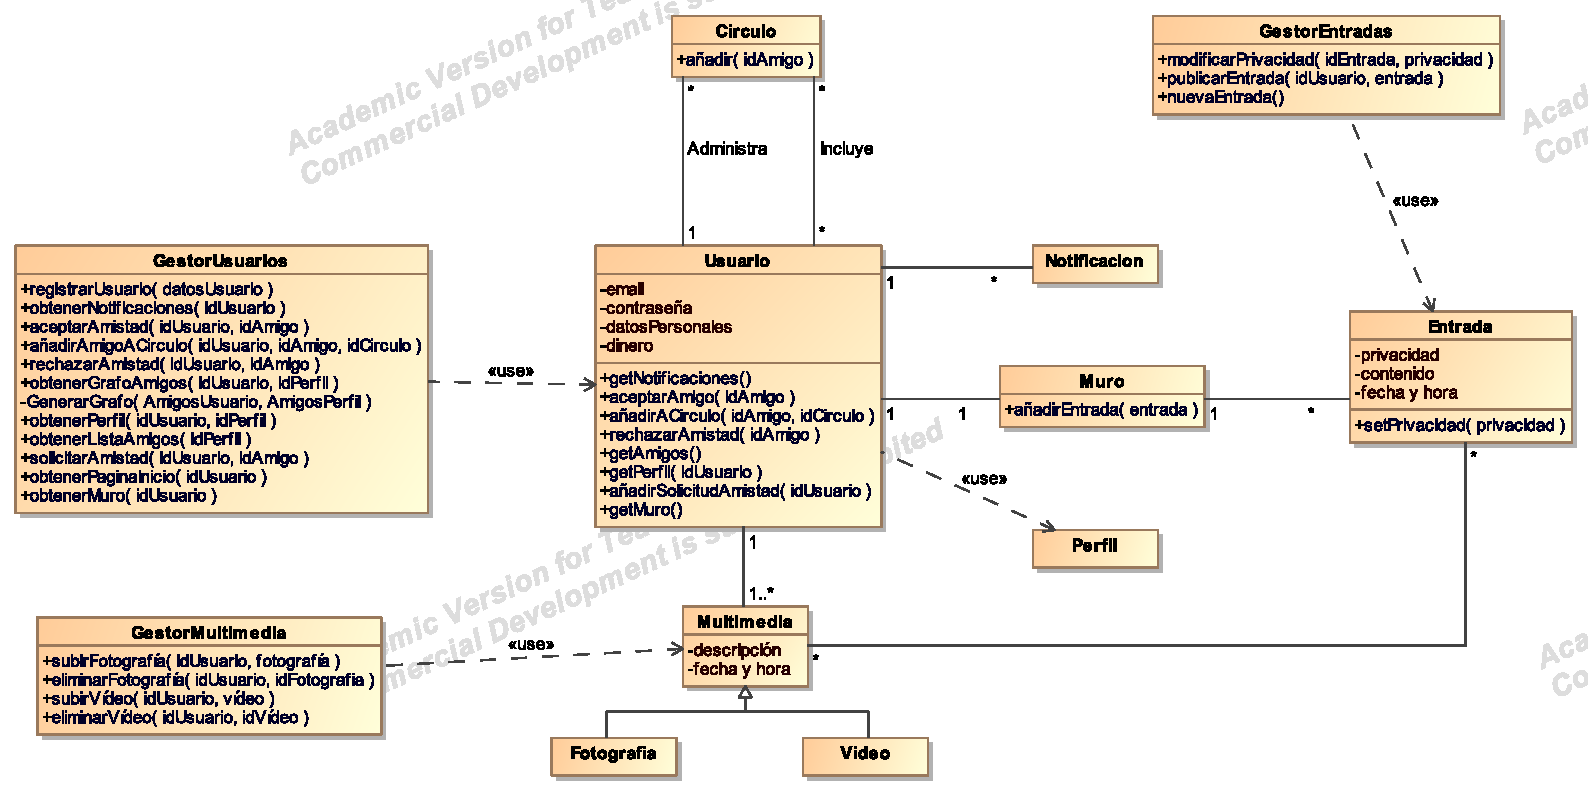
\includegraphics[scale=0.8,angle=90]{Imagenes/DiagramaClases}
	\figcaption{Diagrama de clases}
\end{center}

\end{document}